\documentclass[11pt,border=6pt]{standalone}
\usepackage{fontspec}
\usepackage{tikz}
\usetikzlibrary{positioning,arrows.meta,calc}
\begin{document}
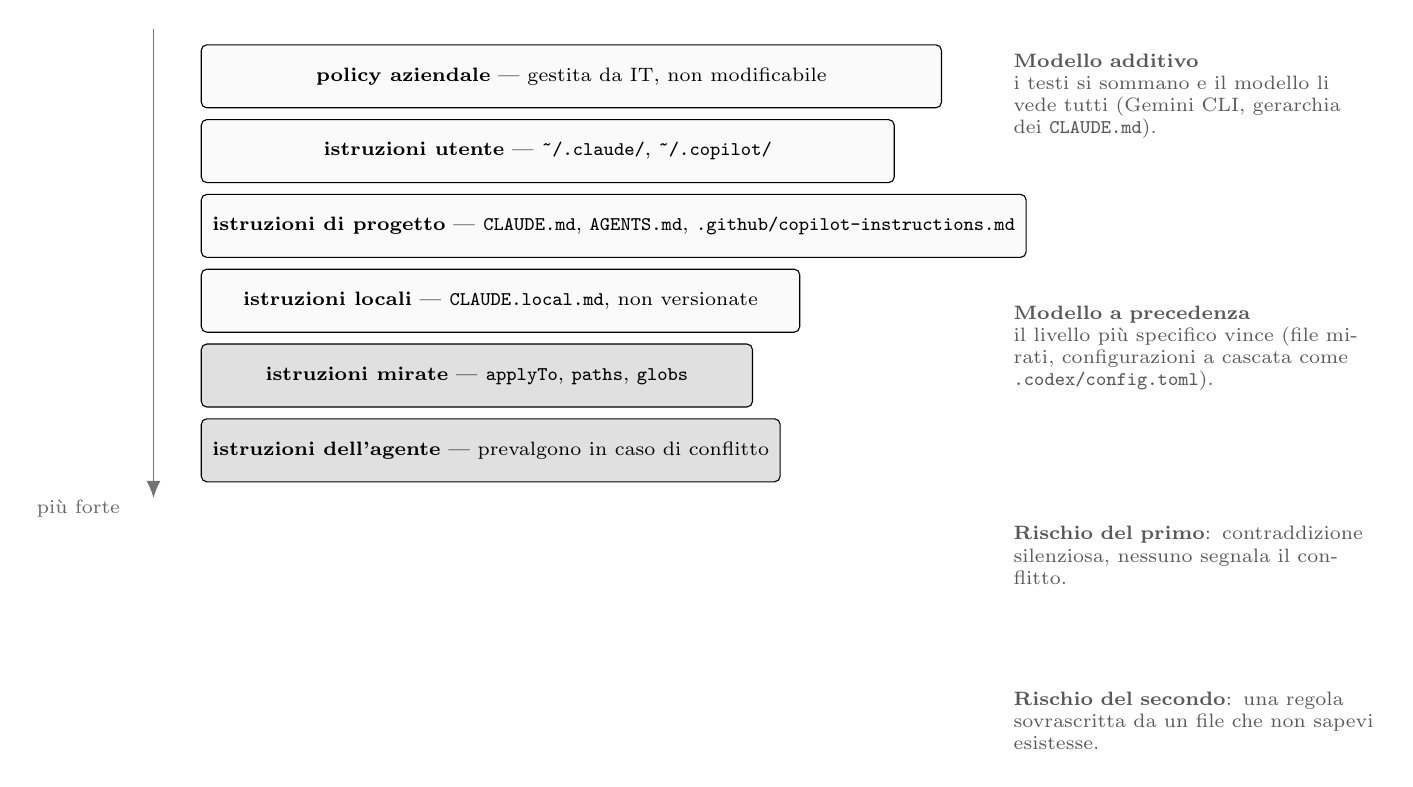
\begin{tikzpicture}[font=\footnotesize,
  lvl/.style={draw, rounded corners=2pt, minimum height=8mm, align=left,
    inner sep=4pt, font=\scriptsize},
  weak/.style={fill=black!2},
  strong/.style={fill=black!12},
  arrow/.style={-{Latex[length=2.2mm,width=1.8mm]}, semithick},
  note/.style={font=\scriptsize, text=black!65, align=left}]

  % barre crescenti: la più specifica è la più stretta e la più forte
  \node[lvl, weak,   minimum width=9.4cm,  anchor=west] (p1) at (0,0)     {\textbf{policy aziendale} --- gestita da IT, non modificabile};
  \node[lvl, weak,   minimum width=8.8cm,  anchor=west] (p2) at (0,-0.95) {\textbf{istruzioni utente} --- \texttt{\textasciitilde/.claude/}, \texttt{\textasciitilde/.copilot/}};
  \node[lvl, weak,   minimum width=8.2cm,  anchor=west] (p3) at (0,-1.90) {\textbf{istruzioni di progetto} --- \texttt{CLAUDE.md}, \texttt{AGENTS.md}, \texttt{.github/copilot-instructions.md}};
  \node[lvl, weak,   minimum width=7.6cm,  anchor=west] (p4) at (0,-2.85) {\textbf{istruzioni locali} --- \texttt{CLAUDE.local.md}, non versionate};
  \node[lvl, strong, minimum width=7.0cm,  anchor=west] (p5) at (0,-3.80) {\textbf{istruzioni mirate} --- \texttt{applyTo}, \texttt{paths}, \texttt{globs}};
  \node[lvl, strong, minimum width=6.4cm,  anchor=west] (p6) at (0,-4.75) {\textbf{istruzioni dell'agente} --- prevalgono in caso di conflitto};

  % freccia di forza crescente
  \draw[arrow, black!55] ([xshift=-6mm,yshift=2mm]p1.north west) -- ([xshift=-6mm,yshift=-2mm]p6.south west);
  \node[font=\scriptsize, text=black!60, anchor=north east] at ([xshift=-9mm,yshift=-1mm]p6.south west) {più forte};

  % annotazioni a destra
  \node[note, text width=4.6cm, anchor=north west] (a) at ([xshift=10.2cm]p1.north west)
    {\textbf{Modello additivo}\\i testi si sommano e il modello li vede tutti (Gemini CLI, gerarchia dei \texttt{CLAUDE.md}).};
  \node[note, text width=4.6cm, anchor=north west] at ([yshift=-3.2cm]a.north west)
    {\textbf{Modello a precedenza}\\il livello più specifico vince (file mirati, configurazioni a cascata come\\\texttt{.codex/config.toml}).};

  % rischi
  \node[note, text width=4.6cm, anchor=north west] at ([yshift=-6.0cm]a.north west)
    {\textbf{Rischio del primo}: contraddizione silenziosa, nessuno segnala il conflitto.};
  \node[note, text width=4.6cm, anchor=north west] at ([yshift=-8.1cm]a.north west)
    {\textbf{Rischio del secondo}: una regola sovrascritta da un file che non sapevi esistesse.};
\end{tikzpicture}
\end{document}
